\documentclass[a4paper,11pt]{book}
\usepackage[left=2cm,right=2cm,top=2cm,bottom=2cm]{geometry}
\usepackage[utf8]{inputenc}
\usepackage[spanish,mexico]{babel}

\usepackage{amsmath, amssymb, amsthm}
%\usepackage{mathrsfs}
\usepackage{appendix}
\usepackage{bachelorstitlepageUNAM}
\usepackage{tikz-network}
%\usepackage{minted}	
%pdflatex -synctex=1 -interaction=nonstopmode --shell-escape %.tex


\usepackage{hyperref}
\usepackage{captdef}

\usepackage{psfrag}
\usepackage{graphicx}
%\usepackage{subfig}
\usepackage{color}
\usepackage{multicol} 
\usepackage{wrapfig}

\usepackage{cancel}
\usepackage[usenames,dvipsnames,svgnames,table]{xcolor}
\usepackage{caption}
\usepackage{subcaption}
\renewcommand{\baselinestretch}{1.5}

\usepackage{hyperref}
%\usepackage[hidelinks]{hyperref} 
\hypersetup{
	colorlinks=true,
	linkcolor=blue,
	filecolor=magenta,      
	urlcolor=cyan,
}
\theoremstyle{plain}
\newtheorem{proposición}{Proposición}
\newtheorem{teorema}{Teorema}
\theoremstyle{definition}
\newtheorem{definición}{Definición}
\newtheorem{ejemplo}{Ejemplo}

%%%%%%%%%%%%%%%%%%%%%%%%%%%%%%%%%%%%%%%%PORTADA%%%%%%%%%%%%%%%%%%%%%%%%%%%%%%%%%%%%%%%%%%

\author{Rodrigo Vega Vilchis}
\title{Estabilidad y transiciones de fase en el sistema de Lotka-Volterra generalizado.}
\faculty{Facultad de Ciencias}
\degree{F\'ISICO}
\supervisor{Dr. Sergio Antonio Alcalá Corona}
\cityandyear{Ciudad Universitaria, CDMX, 2024}
\logouni{Escudo-UNAM}
\logofac{Escudo-FCIENCIAS}

\begin{document}



\frontmatter
\maketitle

\begin{flushright}%
	\emph{A mis padres que siempre fueron insistentes en titularme.}\\
	\emph{A mi hermano, esperando ser siempre su buen ejemplo.}
	\thispagestyle{empty}
\end{flushright}

\chapter{Agradecimientos}

\chapter{Resumen}

\tableofcontents
\listoffigures
\listoftables
%\listofalgorithms

\chapter{Introducción}

\mainmatter
\chapter{De lo simple a lo complejo}

Dentro del marco de los sistemas complejos se manejan varias ramas muy interesantes que le dan su esencia, desde los sistemas dinámicos discretos, dinámica no lineal, teoría de redes complejas, termodinámica fuera de equilibrio, modelos basados en agentes, entre otras. Cada una de ellas aporta un valioso contenido al sistema complejo que se quiera estudiar y analizar dependiendo de sus componentes. Delimitar el área de los sistemas complejos aún resulta una labor complicada debido a su gran \textit{diversidad}, sin embargo, se sabe de la existencia de ciertas características que todo sistema complejo comparte. Los sistemas complejos cuentan con entes: \textit{conectados, interdependientes, dependientes del camino, emergentes} entre otros. El presente trabajo tiene como propósito mostrar al lector cada una de estas características con el objeto de estudio que se va a proponer como piedra angular.\\
\\
Para llegar a conocer nuestra piedra angular primero será necesario delimitar las áreas que intervendrán en la discusión constante de este texto. Se ocupará un \textit{sistema dinámico no-lineal} bajo el soporte de una \textit{red compleja}. La Dinámica no lineal es la rama de los sistemas dinámicos continuos en donde el comportamiento del sistema no se rige por la suma de los comportamientos de sus descriptores. Por ejemplo, una neurona y la suma del comportamiento de las neuronas de un cerebro no puede explicar la emergencia de la consciencia. Por otro lado las redes complejas es la extensión de la \textit{teoría de grafos} aplicada a escenarios comunes de la naturaleza y de la vida cotidiana, tales como redes ecológicas, redes sociales, redes comerciales etc. Su importancia radica en las propiedades que se le pueden extraer para interpretar información sobre la estructura de la red y de la red misma.

\section{Revisión de sistemas lineales.}

En los cursos de ecuaciones diferenciales de cuarto semestre\footnote{citar a Blanchard y Devaney} es obligado abordar el tema de los sistemas de ecuaciones diferenciales lineales con el objetivo de explorar en un primer nivel el comportamiento de diversas cantidades que interactúan y evolucionan en el tiempo. Las ecuaciones diferenciales son la herramienta para modelar fenómenos y su evolución en el tiempo; nos permite trazar soluciones que describen su trayectoria. Dicho de otra forma, son la herramienta para anticipar el comportamiento del fenómeno aunque en la vida real no es tan simple como suena.
\begin{definición}
	Un sistema de ecuaciones diferenciales lineales es una colección de $n$ ecuaciones diferenciales interrelacionadas de la forma
	\begin{equation}\label{eqn:sistemaLineal}
		\begin{split}
			\dot{x}_1 &= f_1(x_1(t),...,x_n(t))\\
			\dot{x}_2 &= f_2(x_1(t),...,x_n(t))\\
			\vdots\\
			\dot{x}_n &= f_n(x_1(t),...,x_n(t))
		\end{split}
	\end{equation}
	donde $f:\mathbb{R}^n\to\mathbb{R}$ lineal, continua y diferenciable. No esta demás recordar que para que una función se considerada lineal debe de cumplir para cualesquiera dos vectores $u,v \in\mathbb{R}^n$ y para todo $k\in\mathbb{R}$ satisface:
	\begin{itemize}
		\item [1.] $f(u+v)=f(u)+f(v)$
		\item [2.] $f(ku)=kf(u)$
	\end{itemize}
	A este cumplimiento se le conoce como \textit{principio de superposición} y el concepto se extiende cuando contamos con las soluciones del sistema lineal.
\end{definición}
Al tratarse de un sistema lineal, resulta bastante oportuno expresarlo en términos de notación matricial, es decir, una multiplicación de una matriz cuadrada $M\in\mathcal{M}_n(\mathbb{R})$ por un vector columna que tiene a todas las funciones $x_i(t)$ lineales.
\begin{align*}
	\begin{split}
			\dot{x}_1 &= a_{11}x_1(t)+\cdots+a_{1n}x_n(t)             \\
			\vdots &\qquad \vdots\qquad\qquad\vdots\qquad\quad\vdots  \\
			\dot{x}_n &= a_{n1}x_1(t)+\cdots+a_{nn}x_n(t)             
	\end{split}	          
	\qquad\ \ \, \Longleftrightarrow
	\begin{split}
		\underbrace{\begin{pmatrix}
				\dot{x}_1\\
				\vdots\\
				\dot{x}_n
		\end{pmatrix}}_{\dot{X}(t)}=\underbrace{\begin{pmatrix}
				a_{11} & \cdots & a_{1n}\\
				\vdots & \ddots & \vdots\\
				a_{n1} & \cdots & a_{nn}
		\end{pmatrix}}_{M}\underbrace{\begin{pmatrix}
		x_1(t)\\
		\vdots\\
		x_n(t)
	\end{pmatrix}}_{X(t)}
	\end{split} 
\end{align*}
en este caso las constantes de la matriz $a_{ij}\in M$ son parámetros que describen ciertas interacciones con respecto de las cantidades que intervienen en el sistema (\ref{eqn:sistemaLineal}); estas interacciones son las responsables de la dinámica del sistema, es decir, de la manera en que evoluciona en el tiempo dependiendo de sus condiciones iniciales. Es conveniente poder contar con la matriz de coeficientes ya que por si sola nos servirá para darle solución al sistema lineal y para poder conocer la estabilidad del mismo, aún sin saber la solución general. Para ahondar en el tema de la estabilidad es necesario conocer los \textit{puntos fijos} del sistema.


%%%%%%%%%%%%%%%%%%CHECHPOINT


\subsection{Puntos fijos y estabilidad del sistema.}

También llamados puntos de equilibrio son aquellos en donde las soluciones de (\ref{eqn:sistemaLineal}) permanecen constantes en el tiempo y dependiendo de su naturaleza\footnote{dictada por los elementos de la matriz de coeficientes $M$.} se establecerá si el punto y el sistema en cuestión es estable o inestable. Para poder hallarlos es necesario hacer cumplir el siguiente sistema de ecuaciones
\begin{equation*}
	\begin{split}
		\dot{x}_1 &= f_1(x_1(t),...,x_n(t))=0\\
		\dot{x}_2 &= f_2(x_1(t),...,x_n(t))=0\\
		\vdots\\
		\dot{x}_n &= f_n(x_1(t),...,x_n(t))=0
	\end{split}
	\quad\Longleftrightarrow\quad
	\begin{split}
		\begin{pmatrix}
			a_{11} & \cdots & a_{1n}\\
			\vdots & \ddots & \vdots\\
			a_{n1} & \cdots & a_{nn}
		\end{pmatrix}
		\underbrace{\begin{pmatrix}
				x_1(t)\\
				\vdots\\
				x_n(t)
		\end{pmatrix}}_{X_0}=0
	\end{split}
\end{equation*}
Para darle solución es necesario encontrar $X_0\in\mathbb{R}^n$ que lo satisfaga; en dicho caso se establece que $X_0$ es el punto fijo del sistema. Los puntos fijos son clave para entender la estabilidad de (\ref{eqn:sistemaLineal}), servirán de referencia para determinar si las soluciones tienden hacia el punto fijo o si divergen del mismo (o una combinación de ambas). Pero tan solo con determinarlo no es suficiente, para ello debemos manipular la matriz de coeficientes $M$ para saber la naturaleza de este punto fijo. Para ello necesitamos hallar los \textit{valores propios} de $M$, por tanto necesitamos determinar
\begin{equation}\label{eqn:vPropios}
	\det(M-\lambda I)=0
\end{equation}
resolviendo el polinomio característico de grado $n$ (dependiendo del tamaño del sistema), se obtendrá el conjunto de valores propios que por si mismos nos brindan demasiada información acerca de como se comportan las soluciones del sistema.

%%%%%%%%%%%%%%%%%%CHECKPOINT
\begin{proposición}\label{prp:Atractores}
	Un sistema lineal que tiene eigenvalores con parte real negativa siempre será estable, es decir, todas las soluciones tenderán hacia el punto fijo del sistema. Este punto de equilibrio del sistema con estas características es conocido como \textbf{Atractor}.
\end{proposición}
Independientemente de la elección de las condiciones iniciales, las soluciones tenderán hacia el punto fijo cuando $t\to\infty$ y se mantendrá ahí siendo resistente ante perturbaciones. Notemos que en la ec. (\ref{eqn:vPropios}) es posible tener raíces reales como complejas, dependiendo de los coeficientes de $M$. Sin embargo aunque se tengan eigenvalores complejos, la dinámica seguirá siendo la misma: se tendrán soluciones que tienden o divergen (o combinación de ambas) del punto fijo, lo que cambia es la forma en que lo hacen. Cuando las soluciones del sistema lineal divergen del punto fijo, entonces se establece que el sistema es inestable y el punto fijo asociado se le conoce como \textbf{\textit{Repulsor}}. Cualquier mínima perturbación que tenga la solución que esta ubicada en el punto fijo, hará que diverga. La combinación de los anteriores se les conoce como \textbf{\textit{Punto silla}}; se dice que es combinación porque podría acercarse al punto silla pero al hacerlo en algún momento terminará divergiendo. Es considerado también como sistema intestable ya que para $t\to\infty$ cualquier solución no trivial se irá a $\infty$.
\begin{ejemplo}\label{eg:Fuente2x2}
	Veamos un ejemplo sencillo para poder apreciar lo anterior, para ello se propone el siguiente sistema de $2\times 2$.
	$$
		\dot{X}(t)=\underbrace{\begin{pmatrix}
				2 & 2\\
				1 & 3
		\end{pmatrix}}_{M_1}X(t)
	$$
	Sacando su polinomio característico (\ref{eqn:vPropios}) tenemos los siguiente eigenvalores\footnote{para sistemas de $2\times 2$ se tiene establecido un polinomio característico que se define como $p_M(\lambda)=\lambda^2-\lambda\text{Tr}A+\det A$}
	\begin{align*}
		p_{M_1}(\lambda)&=\lambda^2-5\lambda+4 = 0\\
		\lambda_1=4 &\qquad \lambda_2=1
	\end{align*}
	Según lo que establece la Proposición \ref{prp:Atractores}, este no es un sistema que sea estable ya que sus eigenvalores tienen parte real positiva. Para poder comprobarlo necesitamos determinar la solución general del sistema asociado a $M_1$. Para ello es necesario encontrar los \textit{eigenvectores} del sistema, es decir
	\begin{align*}
		M_1\vec{v}=\lambda\vec{v}\qquad&\Longleftrightarrow\qquad (M_1-\lambda I)\vec{v}=0 \\
		\vec{v}_{\lambda_1} = \begin{bmatrix}
			1\\
			1
		\end{bmatrix}  \qquad&\qquad \vec{v}_{\lambda_2} = \begin{bmatrix}
		\frac{1}{2}\\
		-1
		\end{bmatrix}
	\end{align*}
\end{ejemplo}
\begin{teorema}\label{teo:Solgral}
	Sea $\vec{v}_0$ un eigenvector de $M$ una matriz asociada al eigenvalor $\lambda$. Entonces la función $X(t)=e^{\lambda t}\vec{v}_0$ es una solución del sistema $\vec{X}(t)=MX(t)$\footnote{ver demostración en el apéndice \ref{ch:Ap}}.
\end{teorema}
Se dice que es una solución general porque podemos seleccionar cualquier $k\in\mathbb{R}$ de tal manera que sea un múltiplo del eigenvector del sistema. En ese caso obtenemos toda una familia de soluciones posibles. Por tanto para el sistema del Ejemplo \ref{eg:Fuente2x2} se tienen las siguientes soluciones posibles:
$$X_1(t)=k_1e^{4t}\begin{bmatrix}
	1\\
	1
\end{bmatrix},\qquad\qquad X_2(t)=k_2e^{t}\begin{bmatrix}
\frac{1}{2}\\
-1
\end{bmatrix}$$
Sin embargo por tratarse de un sistema lineal, se cumple el principio de superposición lo cual significa que la solución general al sistema asociado a $M_1$ es
$$X(t)=k_1e^{4t}\vec{v}_{\lambda_1}+k_2e^{t}\vec{v}_{\lambda_2}$$
Se puede apreciar que para las soluciones separadas y la solución general del sistema asociado a $M_1$, el límite de $X(t)$ cuando $t\to\infty$ es infinito, por tanto las soluciones del Ejemplo \ref{eg:Fuente2x2} siempre van a diverger a infinito independientemente de la elección de condiciones iniciales. Cuando se trata de sistemas lineales, una solución y la suma de las soluciones siempre será solución del sistema, es decir, se pueden escribir como combinación lineal. Generalizando el concepto a un sistema de $n$ ecuaciones lineales tenemos la siguiente solución general:
\begin{equation}\label{eqn:solGral}
	X(t)=k_1e^{\lambda_1 t}\vec{v}_{\lambda_1}+k_2e^{\lambda_2 t}\vec{v}_{\lambda_2}+\cdots+k_ne^{\lambda_n t}\vec{v}_{\lambda_n}
\end{equation}
Esta solución general también aplica perfectamente para el caso en donde se tienen eigenvalores complejos, solamente que habría que descomponer mediante la relación de Euler las exponenciales, es decir, $e^{\lambda t}$ donde $\lambda=a\pm bi$ se descompone como $e^{at}\left (\cos bt+i\sin bt\right )$. Como solución se vería de la siguiente manera
\begin{equation}\label{eqn:solCompleja}
	X(t)=e^a\left (\cos bt+i\sin bt\right )\vec{v}_{\lambda}
\end{equation}
donde $\vec{v}_{\lambda}$ es un vector propio del sistema. Finalmente, en este punto tenemos todos los elementos para darle respuesta a nuestra Proposición \ref{prp:Atractores}; tanto la ecuación (\ref{eqn:solGral}) como (\ref{eqn:solCompleja}) se puede notar que si la parte real del eigenvalor del sistema es positivo, para $t\to\infty$ la exponencial también tiende a infinito y por lo tanto la solución lo hará. En contra parte, si la parte real del eigenvalor es negativa entonces la solución va a tender hacia donde los vectores propios se dirijan, particularmente hacia el punto fijo. Esto únicamente será válido si todos los eigenvalores del sistema tienen parte real negativa ya que si existe al menos uno que tenga parte real positiva eventualmente terminará divergiendo. Eso es lo que sucede con los puntos silla, quizás existan mayoría de eigenvalores con parte real negativa pero si existe al menos uno que tenga parte real positiva, eventualmente para tiempos largos la solución va a diverger. Para poder darnos una idea visual de lo que llamamos \textit{atractores}, \textit{repulsores} y \textit{puntos silla} podemos acceder al espacio fase del sistema y ver de manera integral como se comportan las soluciones del sistema lineal.

\subsection{Espacios fase}

El espacio fase es considerado como la representación geométrica de las trayectorias posibles en un sistema dinámico, en el mismo se contemplan todas las condiciones iniciales posibles y todas las trayectorias posibles que emergen de las anteriores. Aquí mismo encontramos gráficamente los puntos fijos y podemos distinguirlos cualitativamente de que naturaleza son. Las técnicas analíticas descritas anteriormente nos sirven para conocer el comportamiento sin el uso del espacio fase, pero para sistemas de $n=2,3$ podemos acceder al espacio fase y ver como son sus trayectorias. En ese sentido para sistemas con $n>3$ ecuaciones ya será imposible generar su visualización ya que cada uno de los ejes representa una de las cantidades del sistema. \\
\\
En esta breve sección únicamente veremos diversos ejemplos de sistemas $2\times 2$ con eigenvalores variados que nos muestren atractores, repulsores y puntos silla. Sin embargo se omitirán los cálculos de eigenvalores, eigenvectores y soluciones generales, únicamente se pretende mostrar al lector como podemos analizar los sistemas de manera cualitativa a través de sus espacios fase. Por último se dividirán entre espacios fase con eigenvalores reales y con eigenvalores complejos para tener una demarcación adecuada de ambos casos.
\newpage
\begin{ejemplo}
	hola
	
	\begin{figure}[h!]
		\centering
		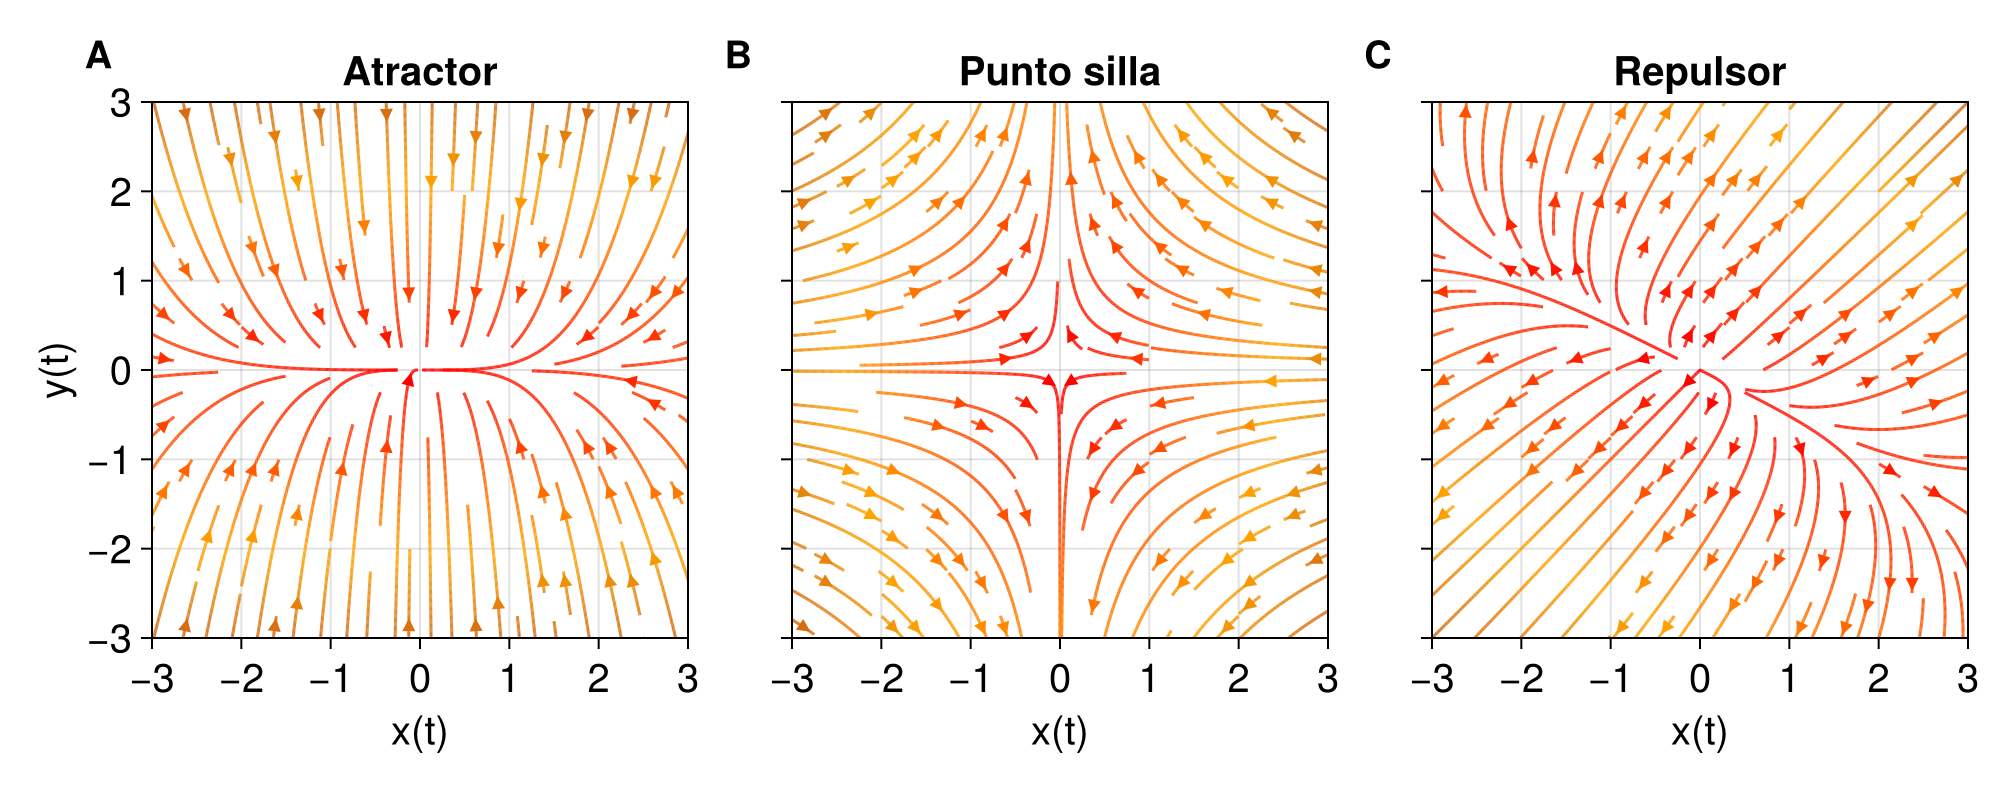
\includegraphics[scale=0.23]{../../Imagenes/Espacios fase reales}
		\caption{Espacios fase con eigenvalores reales.}
	\end{figure}
\end{ejemplo}

\begin{ejemplo}
	hola de nuevo 
	
	\begin{figure}[h!]
		\centering
		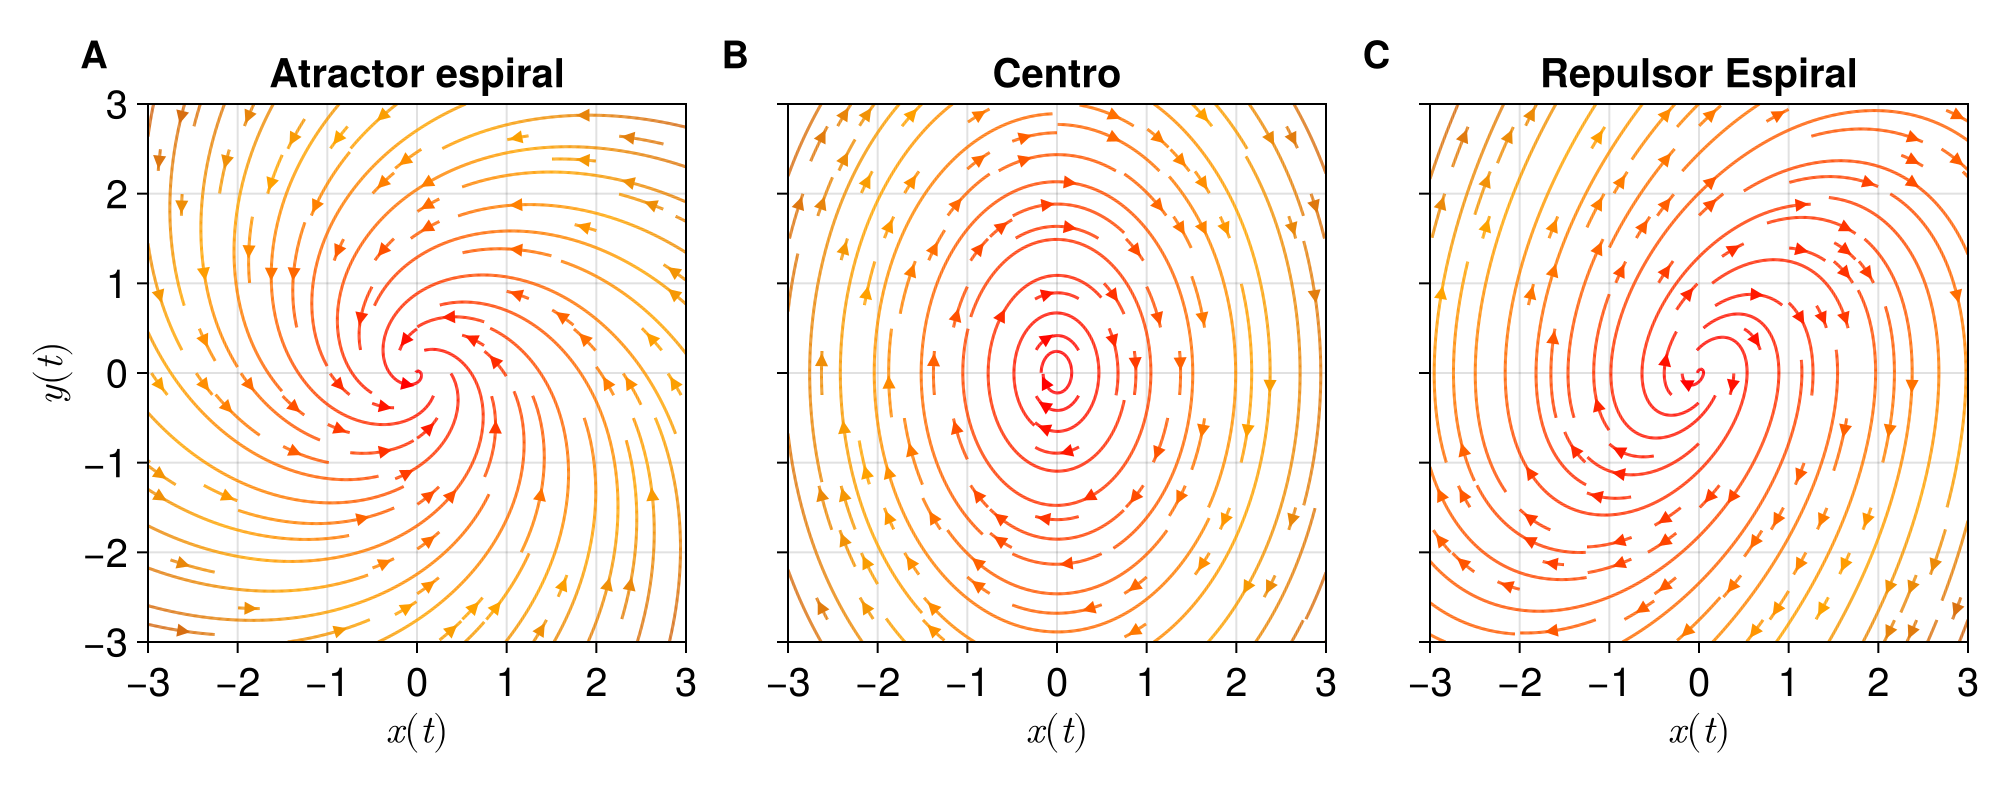
\includegraphics[scale=0.23]{../../Imagenes/Espacios fase complejos}
		\caption{Espacios fase con eigenvalores complejos.}
	\end{figure}
\end{ejemplo}




%%la particularidad con los sistemas no lineales es el hecho de que no se pueden expresar como la suma de las soluciones del sistema, en otras palabras no cumplen el principio de superposición.
\chapter{Estabilidad y transiciones de fase de un sistema complejo.}

El sistema de Lotka-Volterra es uno de los sistemas utilizados para poder comprender la naturaleza de la dinámica no lineal. En este caso particular, los términos no lineales son cuadráticos y representan la interacción entre la especie $i$ y la especie $j$. 
\begin{equation}\label{eqn:LK}
	\frac{dx_i}{dt}=r_ix_i\left(1-\frac{\sum_{j=1}^N \alpha_{ij}x_j}{K_i}\right)
\end{equation}
Se considera una tasa de crecimiento $r_i$ para la especie $i$, una capacidad de carga $K_i$ que limita hasta cierto punto su crecimiento, y su respectiva interacción con la especie $x_j$ cuya ``fuerza'' de interacción esta dada por los coeficientes $\alpha_{ij}$. Al ser un sistema de ecuaciones diferenciales no lineales, no es posible acceder a una solución analítica general\footnote{debido a los términos no lineales... (me gustaría una explicación más completa: ver strogatz y tratados de ecuaciones diferenciales).}; por ello se recurre a métodos de integración numérica capaces de aproximar las soluciones a un rango considerable y cercano a la solución real. El método empleado por excelencia en este trabajo es el integrador Runge-Kutta de orden 4\footnote{poner una referencia de libro}.\\
\\
De manera pedagógica, para aprender y analizar las virtudes y comportamientos del sistema \ref{eqn:LK} es recomendable comenzar explorando el sistema de $2\times 2$.
$$
\begin{cases}
	\dot{x}_1&=r_1x_1(1-\frac{a_{11}x_1}{k_1}-\frac{a_{12}x_1x_2}{k_1})\\
	\dot{x}_2&=r_2x_2(1-\frac{a_{21}x_1x_2}{k_2}-\frac{a_{22}x_2}{k_2})
\end{cases}
$$
En este caso particular, tenemos una tasa de crecimiento y una capacidad de carga personalizada para cada especie, lo que es razonable con el hecho de que cada especie crece a un ritmo determinado y también es limitada de manera determinada. En este caso los coeficientes $\alpha_{ij}$ forman parte de una matriz de \textit{incidencias} entre especies definida de la siguiente manera
\begin{equation}\label{eqn:mIncidencias}
	A=
	\begin{pmatrix}
		1 & \alpha_{12}\\
		\alpha_{21} &1
	\end{pmatrix}
\end{equation}
Es apreciable que los términos de la diagonal se encuentran en $\alpha_{ii} = 1$\footnote{Argumentar más adelante.} respectivamente, más adelante se dará una explicación detallada de esta característica; por el momento solo nos enfocaremos en la dinámica que produce el sistema. Para ello se define el siguiente sistema
\begin{align*}
	\frac{dx}{dt}&=2x\left(1-\frac{x}{2}\right)-xy\\
	\frac{dy}{dt}&=3y\left(1-\frac{y}{3}\right)-2xy
\end{align*}
De este sistema se pueden notar algunas características: se tiene para cada ecuación diferencial (especie) una tasa de crecimiento y una capacidad de carga específica o personalizada. Por ejemplo para la ecuación $\dot{x}$ se tiene una tasa de crecimiento y capacidad de carga de 2 para la especie $x$ y para la especie $y$ estos valores son iguales a 1; para la ecuación $\dot{y}$ se tiene una tasa de crecimiento y capacidad de carga de 3 para la especie $x$ y para la especie $y$ se tiene una tasa de crecimiento de 2 y una capacidad de carga de 1. Aunque este sistema tal cual no tiene una solución analítica per se, si es posible explorar acerca de su comportamiento; en principio se pueden hallar sus puntos fijos que nos hablan de la estabilidad del sistema. Para hallar puntos fijos es necesario encontrar las raíces de este sistema. La solución trivial siempre será $(0,0)$, de ahí se tienen que igualar a cero las ecuaciones para hallar los otros puntos críticos.
\begin{align*}
	2x-x^2-xy &= 0,\qquad\text{suponiendo que $y = 0$}\\
	2x &= x^2\\
	x&=2
\end{align*}
y para $\dot{y}$ se tiene
\begin{align*}
	3y-y^2-2xy&=0,\qquad\text{suponiendo que $x=0$}\\
	3y &= y^2\\
	y &= 3
\end{align*}
Por tanto tenemos para $\dot{x}$ el punto fijo $(2,0)$ mientras que para $\dot{y}$ se tiene el punto fijo $(0,3)$. Aún es posible hallar un último punto fijo que es para cuando ambas ecuaciones se hacen cero.
\begin{align*}
	2x-x^2-xy&=0,\qquad\text{Se despeja $y$ de esta ecuación.}\\
	xy &= x(2-x)\\
	y &= (2-x)\\
	\\
	3(x-2)-(x-2)^2-2x(x-2) &= 0\\
	3x-6-(x^2-4x+4)-2x^2+4x&=0,\qquad\text{Reduciendo términos se tiene.}\\
	x^2-3x+2 &= 0
\end{align*}
%%%%%%%%%%%%%%%%%%%%%CHECKPOINT
Al resolver esta última ecuación se determina el último punto fijo que corresponde a $(1,1)$. Los puntos fijos brindan información para explorar hacia donde pueden converger (atractores) o diverger (repulsores o puntos sillas) las soluciones del sistema dependiendo de las condiciones iniciales que se le impongan.\footnote{explicar brevemente de que se trata uno, quizás esto deba precisarse desde la introducción.} Se establece que si las soluciones convergen entonces el sistema es considerado \textit{estable} mientras que 
\begin{wrapfigure}{r}{0.5 \textwidth} \vspace{-30pt} \begin{center}
		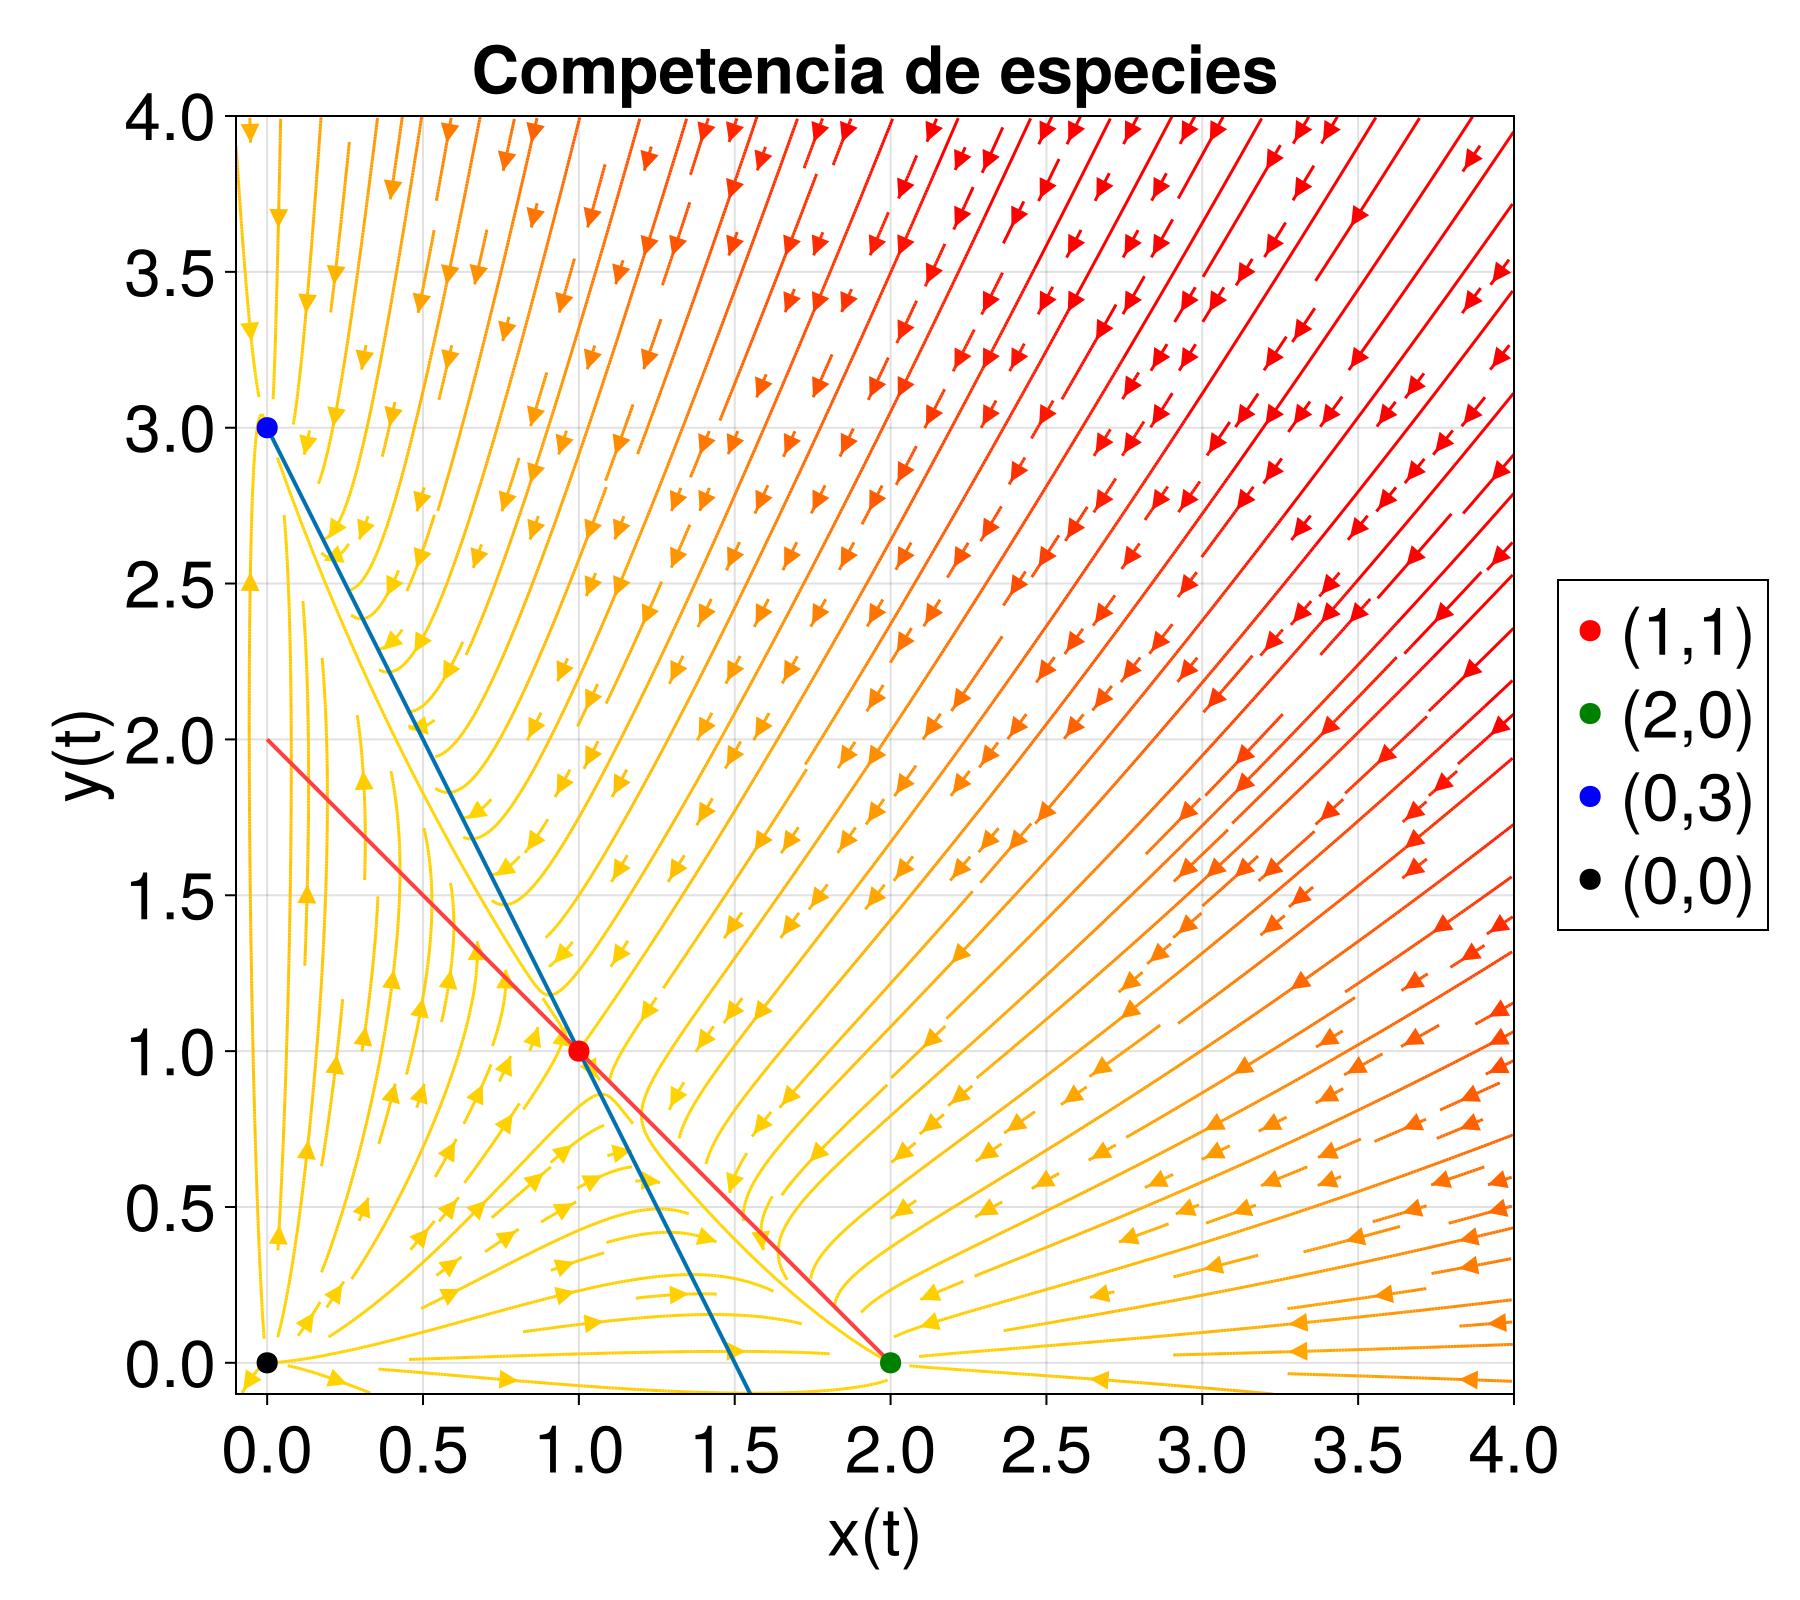
\includegraphics[width=0.5\textwidth]{../../Imagenes/Competencia de especies} 
	\end{center} 
	\vspace{-20pt} 
	\caption{Campo vectorial de las soluciones del sistema propuesto de dos especies.} 
	\vspace{-10pt}
	\label{fig:CompetenciaEspecies}
\end{wrapfigure} 
en caso contrario el sistema es considerado \textit{inestable.} Es posible determinar mediante técnicas computacionales el campo vectorial de las soluciones de este sistema\footnote{Realizar referencia de la técnica empleada.}, inclusive dos de las isoclinas\footnote{si son isoclinas???} del sistema resolviendo las ecuaciones igualando a cero y despejando $y$ de cada una de ellas. Es notorio como dichas isoclinas inciden de alguna forma en tres de los puntos fijos. El gráfico nos muestra que las soluciones convergen hacia los puntos que se encuentran en los ejes; todo dependerá de las condiciones iniciales del sistema para ver hacia donde convergen. El punto fijo de en medio es conocido como punto silla y es inestable ya que aunque existan soluciones que convergan hacia él mismo, en la mínima perturbación que se le provoque la solución puede ``desviarse'' hacia los atractores. Por último se observa que del origen divergen todas las soluciones por lo que es considerado un punto fijo repulsor.\\
\\
%%%%%%%%%%%%%%%%%%%%%CHECKPOINT
%% Nada más checar la aseveración de las isoclinas para ver si se queda o se retira del párrafo
En esta ocasión por tratarse de un sistema de $2\times 2$, se tuvo la fortuna de poder obtener una representación visual del sistema y poder realizar un análisis cualitativo del mismo para sacar conclusiones. Pero ¿qué sucede cuando se tienen sistemas de $N$ especies? En principio el espacio vectorial (fase) de las soluciones se vuelve $N-$dimensional y por lo tanto imposible de visualizar en un gráfico. Es por ello que se requieren de otras técnicas analíticas para seguir esbozando el comportamiento del sistema. Una herramienta útil a esta conjetura es la de \textit{linealizar}\footnote{Explicar brevemente en esta nota a que se refiere esto.} el sistema para poder explorar el comportamiento de los puntos fijos a nivel local. Para realizar esta acción es necesario aplicar el \textit{Jacobiano} al sistema para ``bajar'' el grado de las ecuaciones del sistema \ref{eqn:LK} y así obtener puras ecuaciones lineales.\\
\\
Se define la función vectorial $\mathbf{F}:\mathbb{R}^n\to\mathbb{R}^n$, donde $n$ será el número de especies del sistema de Lotka-Volterra generalizado \ref{eqn:LK}.
\begin{equation}\label{eqn:Fmatricial}
	\mathbf{F}(\vec{x})=\begin{pmatrix}
		\dot{x}_1=f_1(\vec{x})\\
		\vdots\\
		\dot{x}_n=f_n(\vec{x}))
	\end{pmatrix},\qquad\text{donde $\vec{x}(t)=\left(x_1(t),...,x_n(t))\right)\in\mathbb{R}^n$.}
\end{equation}
Las componentes de $\mathbf{F}(\vec{x})$ corresponden con las funciones del sistema \ref{eqn:LK}, y las componentes del vector $\vec{x}$ corresponden con sus especies involucradas. El sistema \ref{eqn:LK} puede ser re-escrito bajo la simplicidad de la siguiente ecuación
\begin{equation}\label{eqn:LKmatricial}
	\dot{X}(t) = \mathbf{F}(X(t)),\qquad\text{considerando $\dot{X}(t)=\frac{d\vec{x}(t)}{dt}$}
\end{equation}
Por tanto el Jacobiano del sistema se definirá de la siguiente manera
\begin{equation}\label{eqn:Jacobiano}
	\mathbb{J}_\mathbf{F}(\vec{x}) = \begin{pmatrix}
		\frac{\partial f_1(\vec{x})}{\partial x_1} & \cdots &\frac{\partial f_1(\vec{x})}{\partial x_n}\\
		\vdots & \ddots & \vdots\\
		\frac{\partial f_n(\vec{x})}{\partial x_1} & \cdots &\frac{\partial f_n(\vec{x})}{\partial x_n}
	\end{pmatrix}
\end{equation}
Esta resultante al ser evaluada en los puntos fijos del sistema genera la llamada matriz de \textit{interacciones} que es aquella que nos brinda la información necesaria para determinar la estabilidad de ese punto fijo en particular. Por ello se establece que la matriz de interacciones brinda información solo a nivel local, pues no contiene información de otros puntos fijos ajenos. Para validar esta aseveración ocuparemos nuestro sistema de $2\times 2$ y relacionaremos la matriz de interacciones con lo que se muestra en el gráfico. El Jacobiano del sistema \ref{eqn:LK} para $n=2$ es el siguiente
\begin{equation}\label{eqn:Jacobiano2}
	\mathbb{J}_\mathbf{F}(\vec{x})=\begin{pmatrix}
		r_1-\frac{2r_1x_1+r_1a_{12}x_2}{K_1} & -\frac{r_1a_{12}x_1}{K_1}\\
		-\frac{r_2a_{21}x_2}{K_2} & r_2-\frac{2r_2x_2+r_2a_{21}x_1}{K_2}
	\end{pmatrix}
\end{equation}
debido a la matriz de incidencias \ref{eqn:mIncidencias}, se tiene que los valores $a_{ii}=1$ que corresponden con las auto-interacciones. Evaluando los puntos fijos antes encontrados en el jacobiano \ref{eqn:Jacobiano2} se tienen las siguientes matrices de interacciones:
$$
\mathbb{J}_{(2,0)} = \begin{pmatrix}
	-2 & -2\\
	0 & -1
\end{pmatrix},\qquad \mathbb{J}_{(0,3)}=\begin{pmatrix}
	-1 & 0\\
	-6 & -3
\end{pmatrix},\qquad \mathbb{J}_{(1,1)}=\begin{pmatrix}
	-1 & -1\\
	-2 & -1
\end{pmatrix},\qquad \mathbb{J}_{(0,0)}=\begin{pmatrix}
	2 & 0 \\
	0 & 3
\end{pmatrix}
$$
%%%%%%%%Checkpoint
Como previamente se ha revisado\footnote{Hay que referenciar este enunciado con algún sustento de la introducción en donde se maneje el tema de los eigenvalores y eigenvectores como solución de sistemas lineales.}, los eigenvalores (más que los eigenvectores) determinan la estabilidad de un sistema lineal. Se establece que mientras ellos tengan parte real negativa se asegurará que el sistema será estable y que en otro caso el sistema será inestable. Por lo tanto los eigenvalores de las primeras dos matrices de interacciones deben ser negativos para que sustenten los atractores de la figura \ref{fig:CompetenciaEspecies}. Mientras que los eigenvalores de $\mathbb{J}_{(1,1)}$ deben ser uno negativo y otro positivo para sustentar al punto silla. Para la matriz $\mathbb{J}_{(0,0)}$ sus eigenvalores deben ser positivos para que sustenten el repulsor. Realizando el álgebra correspondiente se encuentra lo siguiente
\begin{align*}
	\mathbb{J}_{(2,0)}&\Longrightarrow\ \lambda_1 = -2,\quad\lambda_2 = -1\\
	\mathbb{J}_{(0,3)}&\Longrightarrow\ \lambda_1 = -3,\quad\lambda_2 = -1\\
	\mathbb{J}_{(1,1)}&\Longrightarrow\ \lambda_1 = -1+\sqrt{2},\quad\lambda_2 = -1-\sqrt{2}\\
	\mathbb{J}_{(0,0)}&\Longrightarrow\ \lambda_1 = 2,\quad\lambda_2 = 3\\
\end{align*}
Por tanto se termina de validar la consistencia del método de la linearización para esbozar la estabilidad de \ref{eqn:LK} por cada uno de sus puntos fijos. Esta forma analítica de reconocer la estabilidad del sistema será sumamente útil para cuando se tengan $N>3$ especies. Habiendo conocido las técnicas a nivel particular frente al sistema para $n=2$ toca generalizar las ideas hacia un sistema más robusto de $N$ especies, a continuación se abordará esa discusión.

%%%%%%%%% Checkpoint
\subsection{Sistema de competencia de especies generalizado para $N$ especies.}

En la sección anterior se ha introducido el sistema de competencia de especies \ref{eqn:LK} y su forma vectorial \ref{eqn:LKmatricial} generalizada; se mostró un ejemplo particular con $n=2$ para observar su dinámica a través de su espacio fase (fig. \ref{fig:CompetenciaEspecies}) en donde se contempla la naturaleza de sus puntos fijos si se trata de atractores, repulsores o puntos silla. Se propone propone el método de la linearización para conseguir matrices de interacción que determinen de forma analítica la estabilidad de cada uno de los puntos fijos del sistema. En esta sección profundizaremos más acerca de lo mencionado comenzando con la matriz de incidencias \ref{eqn:mIncidencias} la cual ya se ha mencionado anteriormente. \\
\\
Para este trabajo resultó conveniente utilizar el marco de las \textit{redes complejas} para poder representar las interacciones entre las especies del sistema. Una red es considerada una colección de \textit{nodos} que se encuentran unidos por \textit{enlaces}\footnote{definir más adelante el tipo de interacciones con base en el signo y si son dirigidas o no dirigidas. Además de agregar cita del Newman para esta definición.}. Para definir redes siempre es necesario establecer que es lo que representan los nodos y que representan los enlaces, en nuestro caso por ejemplo si existe una interacción entre las especies $x_i$ y $x_j$ (nodos de la red) entonces hay un enlace que los une. Por tanto establecemos que los nodos de la red corresponden con las especies y los enlaces con las interacciones.
\begin{wrapfigure}{l}{0.45 \textwidth} \vspace{-30pt} \begin{center}
		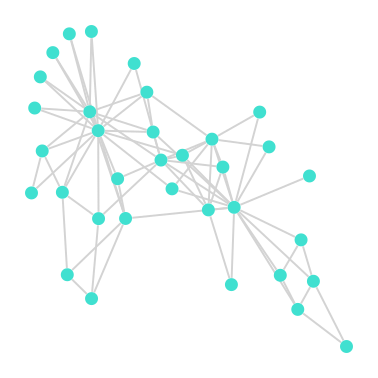
\includegraphics[width=0.45\textwidth]{../../Imagenes/karate} 
	\end{center} 
	\vspace{-20pt} 
	\caption{Red de Karate.} 
	\vspace{-10pt}
	\label{fig:RedKarate}
\end{wrapfigure} 
En el mundo es posible encontrar diferentes tipos de redes con cierto significado, tales como la red de energética de un país, redes de amistades en una universidad o redes de acciones que cotizan en la bolsa de valores. Para poder representar estas redes y cualquier otro tipo de red conviene introducir el concepto de \textit{matriz de adyacencia.}
\begin{definición}\label{def:1}
	Sea $A\in\mathcal{M}_n(\mathbb{R}) $. Se define la matriz de adyacencia tal que sus entradas son de la siguiente forma
	$$a_{ij}= 
	\begin{cases}
		1, \ \text{si $\exists$ un enlace entre el nodo $i$ y el nodo $j$.}\\
		0, \ \text{en otro caso}.
	\end{cases}$$
\end{definición}
%%%%%%% Checkpoint
La matriz de adyacencia será la herramienta para determinar la relación de interacción entre especies, pero solo hablará de su existencia más no tendrá información del peso de dicha interacción. Recordemos que en el sistema \ref{eqn:LK} tenemos coeficientes $\alpha_{ij}$ que representan dichos pesos de interacción entre especies, esto se retomará más adelante. 
\begin{ejemplo}
	Para poder apreciar la matriz de adyacencia definamos una red de 10 nodos y veamos su matriz de adyacencia que le corresponde. Es notorio que cada nodo se encuentra identificado con un número de nodo, esto nos va a servir  para poderlo mapear en la matriz de adyacencia. La correspondencia es la siguiente:
\end{ejemplo}
\begin{wrapfigure}{r}{0.5 \textwidth} \vspace{-30pt} \begin{center}
		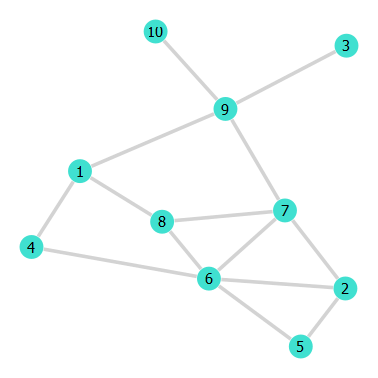
\includegraphics[width=0.45\textwidth]{../../Imagenes/Red10} 
	\end{center} 
	\vspace{-20pt} 
	\caption{Red no dirigida de 10 nodos.} 
	\vspace{-120pt}
	\label{fig:Red10}
\end{wrapfigure} 

$$
A = \begin{pmatrix}
	0 & 0 & 0 & 1 & 0 & 0 & 0 & 1 & 1 & 0\\
	0 & 0 & 0 & 0 & 1 & 1 & 1 & 0 & 0 & 0\\
	0 & 0 & 0 & 0 & 0 & 0 & 0 & 0 & 1 & 0\\
	1 & 0 & 0 & 0 & 0 & 1 & 0 & 0 & 0 & 0\\
	0 & 1 & 0 & 0 & 0 & 1 & 0 & 0 & 0 & 0\\
	0 & 1 & 0 & 1 & 1 & 0 & 1 & 1 & 0 & 0\\
	0 & 1 & 0 & 0 & 0 & 1 & 0 & 1 & 1 & 0\\
	1 & 0 & 0 & 0 & 0 & 1 & 1 & 0 & 0 & 0\\
	1 & 0 & 1 & 0 & 0 & 0 & 1 & 0 & 0 & 1\\
	0 & 0 & 0 & 0 & 0 & 0 & 0 & 0 & 1 & 0\\
\end{pmatrix}
$$
Los renglones y columnas de la matriz representan los nodos, siendo el primer renglón el primer nodo (número 1), el quinto renglón será el quinto nodo (número 5); esto pasa de manera equivalente con las columnas, la cuarta columna corresponde con el cuarto nodo (número 4), la octava columna corresponde con el octavo nodo (número 8). Por tanto, mediante la matriz de adyacencia sabemos que el primer nodo (renglón 1) esta enlazado con el cuarto nodo (columna 4) ya que existe un uno, mientras que el primer renglón y la quinta columna hay un cero lo que indica que no existe un enlace entre estos nodos. \\
\\
También hay que destacar qué la matriz es simétrica y que la diagonal es igual a cero: para el primer punto se debe notar que la relación de los enlaces entre nodos no tiene dirección, es decir, que exista un enlace entre nodos significa que el nodo $i$ se conecta con $j$ y viceversa, que el nodo $j$ se conecta con el nodo $i$. Por tanto decimos que la red de la fig. \ref{fig:Red10} es \textit{no dirigida} puesto que no hay una dirección preferencial en el enlace, esto implica que su matriz de adyacencia es simétrica. Para el segundo punto se debe notar que cada nodo es libre de relacionarse consigo mismo, en este ejemplo los nodos no lo  hacen pero si es posible la existencia de \textit{autoenlaces}; en nuestro sistema tendrá un alto signíficado porque se hablarán de las autointeracciones que son importantes para la construcción del sistema.\footnote{hay que completar esta idea, relacionada con la diagonal de unos. Autointeracción para la existencia del sistema, capacidad de carga. Argumentar bien.}
\\
\\
Cuando se tiene el caso en que los enlaces tienen una dirección preferencial de nodo a nodo, decimos que corresponde a una \textit{red dirigida}. En este caso el enlace podrá ir del nodo $i$ al nodo $j$ pero no necesariamente lo hará en sentido contrario, deberá definirse explícitamente. En el mundo también existe un gran conjunto de redes dirigidas como lo son las citaciones académicas, la propia WWW (World Wide Web), incluso redes tróficas de depredador-presa. Y para este caso también se tiene asociada una matriz de adyacencia con una ligera diferencia con respecto de la definición \ref{def:1}.
\begin{definición}
	Sea $D\in\mathcal{M}_n(\mathbb{R})$, matriz de adyacencia de una red no dirigida. Se definen sus elementos de la siguiente manera:
	$$
	\alpha_{ij}=\begin{cases}
		1,\qquad\text{Si existe un enlace del nodo $i$ al nodo $j$}\\
		0,\qquad\text{otro caso.}
	\end{cases}
	$$
\end{definición}
Los enlaces de las redes dirigidas van a estar representados por flechas para que puedan mostrar adecuadamente las direcciones correspondientes entre los nodos. 
\newpage
\begin{ejemplo}
	Se tiene la siguiente red dirigida de 10 nodos con exactamente 14 enlaces. La matriz de adyacencia asociada es la siguiente
\end{ejemplo}

\begin{wrapfigure}{l}{0.5 \textwidth} \vspace{-30pt} \begin{center}
		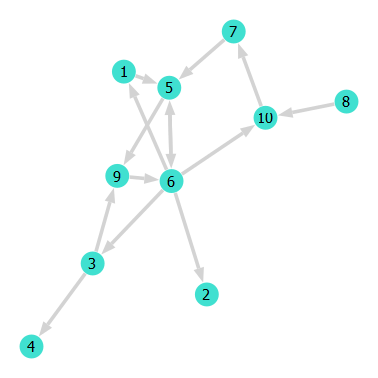
\includegraphics[width=0.45\textwidth]{../../Imagenes/Red10Dir} 
	\end{center} 
	\vspace{-20pt} 
	\caption{Red no dirigida de 10 nodos.} 
	\vspace{-120pt}
	\label{fig:Red10Dir}
\end{wrapfigure} 
$$
D = \begin{pmatrix}
	0 & 0 & 0 & 0 & 1 & 0 & 0 & 0 & 0 & 0\\
	0 & 0 & 0 & 0 & 0 & 0 & 0 & 0 & 0 & 0\\
	0 & 0 & 0 & 1 & 0 & 0 & 0 & 0 & 1 & 0\\
	0 & 0 & 0 & 0 & 0 & 0 & 0 & 0 & 0 & 0\\
	0 & 0 & 0 & 0 & 0 & 1 & 0 & 0 & 1 & 0\\
	1 & 1 & 1 & 0 & 1 & 0 & 0 & 0 & 0 & 1\\
	0 & 0 & 0 & 0 & 1 & 0 & 0 & 0 & 0 & 0\\
	0 & 0 & 0 & 0 & 0 & 0 & 0 & 0 & 0 & 1\\
	0 & 0 & 0 & 0 & 0 & 1 & 0 & 0 & 0 & 0\\
	0 & 0 & 0 & 0 & 0 & 0 & 1 & 0 & 0 & 0\\
\end{pmatrix}
$$




\backmatter
% bibliography, glossary and index would go here.

\end{document}